% !TeX spellcheck = da_DK
\subsection{Patientsikkerhed}
Ved brug af medicinsk udstyr er sikkerheden for patienten vigtig, da de ofte er hæmmede eller svækkede og derfor yderligere følsomme. Patientsikkerhed indebærer fokus på de fysiologiske konsekvenser patienten kan blive udsat for, når de tilkobles elektroniske kredsløb. Hvis ikke patientens sikkerhed er i orden, vil vedkommende opleve at blive en del at det elektroniske kredsløb. Dette kan medføre alvorlige følger, da patienten vil blive udsat for elektrisk strøm. Når elektrisk strøm løber igennem biologisk væv, kan tre fænomener forekomme: modstandsopvarmning af væv, elektrokemiske forbrændinger og elektrisk stimulering af muskel- og nervevæv. [1] 
\begin{figure}[H]
	\centering
	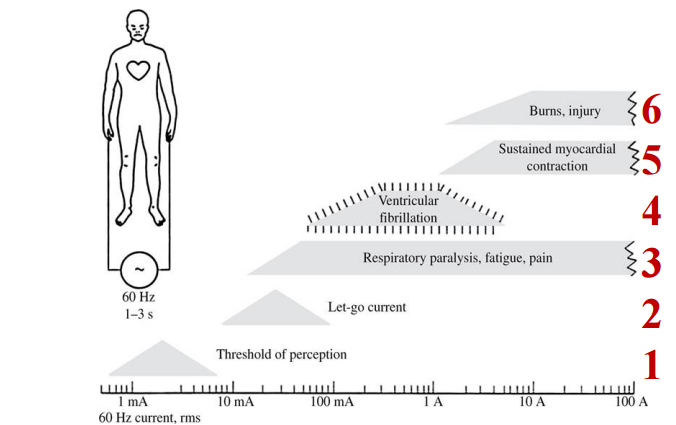
\includegraphics[scale=0.5]{figures/bProblemanalyse/Patientsikkerhed.png}
	\caption{Figuren viser effekten, som strømmen har på patienten ved forskellige strømstyrker og er inddelt i 6 stadier. Figurens gyldighed er forudsat, at personen har en vægt på 70 kg og er i kontakt med et elektronisk kredsløbet i 1-3 sekunder ved 60 Hz med begge hænder. \fxnote{Kilde er Webster2009, men den er ikke lagt ind i JabRef endnu (29/09)}}
	\label{Patientsikkerhed}
\end{figure}

På \figref{Patientsikkerhed} ses den effekt som elektrisk strøm kan have på patienten ved forskellige strømstyrker. Disse effekter kan opdels i seks forskellige stadier.

\textbf{Stadie 1}
 I stadie 1 på \figref{Patientsikkerhed} findes den laveste strømstyrke på 0,5-10 mA. Ved dette stadie vil patienten føle en prikkende fornemmelse. Strømtætheden er stor nok til at aktivere nervesensorerne i huden, hvilket kan give en let opvarmning heraf. 

\textbf{Stadie 2} 
Ved stadie 2 på \figref{Patientsikkerhed} udsættes patienten for en elektrisk strøm mellem 10 mA og 100 mA. Dette er den maksimale strøm, hvor patienten kan afbryde kontakten frivilligt. Patienten vil opleve en kraftig påvirkning af muskler og nerver, hvilket resulterer i muskeltræthed og smerte, da musklerne skal lave ufrivillige kontraktioner.
 
 \textbf{Stadie 3}
I stadie 3 på \figref{Patientsikkerhed} er strømstyrken mellem 20 mA og 100 A og her kan patienten opleve åndedrætslammelser, smerter og muskeltræthed. Dette kan desuden resultere i kvælning, hvis strømmen ikke afbrydes. 

\textbf{Stadie 4}
Ved stadie 4 på \figref{Patientsikkerhed}, som ligger mellem 75 mA og 4 A, kan patienten opleve ufrivillig kontraktion af hjertemuskulaturen, hvilket kan medføre ventrikelflimmer. 

\textbf{Stadie 5}
I det 5. stadie på \figref{Patientsikkerhed} er strømstyrken mellem 1 A og 100 A. Her sker kontraktioner af hele hjertemuskulaturen. Dette kan resultere i hjertestop, da hjertet er konstant kontraheret og derfor ikke kan videregive elektriske signaler. 

\textbf{Stadie 6}
Ved det 6. og sidste stadie på \figref{Patientsikkerhed} vil patienten opleve stærk strøm, som kan medføre alvorlige brandsår på huden. Ved store strømstyrker kan muskelkontraktionerne blive så kraftige, at musklen og knoglerne kan løsrive sig fra hinanden. Derudover vil hjernen og nervevæv miste alle funktioner, når store strømme løber gennem kroppen. Som det ses på \figref{Patientsikkerhed} kan flere af stadierne overlappe hinanden og foregå samtidig. [1]

Der er forskellige muligheder for, hvordan den elektriske strøm løber igennem kroppen, hvilket bestemmer, hvor skadende strømmen er for patienten. De to forskellige muligheder er makro- og mikrochok. Makrochok sker, når strømmen løber igennem kroppen ved to punkter på hudens overflade og derved går kun en mindre del af strømmen igennem hjertet. Mikrochok sker, når det meste af strømmen løber igennem hjertet. Strømmen kommer fra et punkt på hudens overflade og forekommer hos patienter med elektriske ledere i hjertet f.eks. katetere. [1]

Det er vigtigt at have fokus på patientsikkerhed, når der skal fremstilles medicinsk udstyr, som skal tilsluttes patienter. Dette kan gøres med en jordforbindelse i systemet eller ved at sørge for, der ikke er direkte kontakt mellem patienten og elnettet. Store mængder strøm kan have alvorlige konsekvenser for patientens heldbred. 


%[1] - Medical Instrumentation: Application and Design. Webster, John G. 2009.